
\begin{ledgroupsized}[r]{120mm}
\footnotesize
\pstart
\noindent\textbf{Überlieferung:}
\pend
\end{ledgroupsized}
\begin{ledgroupsized}[r]{114mm}
\footnotesize
\pstart
\parindent -6mm
\makebox[6mm][l]{\textit{L}}%
Aufzeichnung:
LH~XXXV~10, 16~Bl.~9. 
Ein Zettel (ca.~15,5~x~9~cm.);
alle Ränder bis auf den unteren beschnitten.
Eine Seite auf Bl.~9~r\textsuperscript{o};
\href{\Scan{LH_35_10_16_009v}}%
{Bl.~9~v\textsuperscript{o}}
leer bis auf zwei Zahlenreihen 
(letzte Ziffern der Vielfachen von 2 bzw. von 3): 
\textit{2 \textbar\ 2 4 6 8 0 \textbar\textbar\ 3 \textbar\ 3 6 9 2 5 8 1 4 7 0}.
\pend
\end{ledgroupsized}
\vspace{5mm}
\begin{ledgroup}
\footnotesize
\pstart
\noindent
\textbf{Datierungsgründe:}
Die Überlegungen in N.\;\ref{60129} knüpfen an 
\indexN{\textls{Stevin} (Stevinus), Simon 1548\textendash1620}Stevins 
berühmten "Kugelkettenbeweis"
für das Gesetz der Zerlegung von Kräften auf schiefen Ebenen an: 
vgl. 
\indexN{\textls{Stevin} (Stevinus), Simon 1548\textendash1620}%
\textsc{S.~Stevin}, \cite{00196}\textit{De Beghinselen der Weeghconst}, Leiden 1586, 
Buch~1, Teil~2,
Theor.~XI Prop.~XIX mit Koroll.~I, S.\;40\textendash42
(\cite{02084}\textit{SPW} I, S.\;174\textendash179).
Neben einem Referat von \indexN{\textls{Stevin} (Stevinus), Simon 1548\textendash1620}Stevins Beweis enthält N.\;\ref{60129} eine Erweiterung des Gesetzes auf eine schiefe krumme Fläche.
\pend
\pstart
Obwohl im bislang edierten Leibnizkorpus sich keine Erwähnungen finden, die  den Zeitpunkt der ersten Lektüre der statischen Werke \indexN{\textls{Stevin} (Stevinus), Simon 1548\textendash1620}Stevins eindeutig bestimmen ließen, so darf dennoch von einer sehr frühen Begegnung Leibnizens mit diesem allgemein bekannten Satz ausgegangen werden. 
Des Weiteren stellt N.\;\ref{60129} wohl keinen direkten Zeugen der ersten Lektüre von Stevin dar, 
da es sich einerseits beim Referat des Beweises nicht um einen Auszug aus der niederländischen \cite{00196}Erstausgabe von 1586 handelt,
noch aus der von 
\indexN{\textls{Snell van Royen} (Snellius), Willebrord 1580\textendash1626}W.~Snell 
besorgten lateinischen Übersetzung (\cite{02130}\textit{Hypomnemata Mathematica}, Leiden 1605\textendash1608, tom.~4, S.\;34\,f.);
und andererseits Leibniz \indexN{\textls{Stevin} (Stevinus), Simon 1548\textendash1620}Stevins Gedanken eigens weiterführt.
\pend
\pstart
Einen möglichen Anhaltspunkt
für die Datierung von N.\;\ref{60129}
bieten indessen die wahrscheinlich um 1680 verfassten Konzepte 
"Principium Mechanicae universae novum"
(LH~XXXV~10, 5 Bl.~1\textendash4, Fortsetzung in LH~XXXVII~5, Bl.~178\textendash179 und LH~XXXVII~5 Bl.~53\textendash54),
die der Begründung des \textit{principium aequilibrii} auf verschiedenen Gebieten der Mechanik gewidmet sind (die Texte werden in einem späteren Band der Reihe erscheinen). Für die Begründung der Anwendung in der Statik beruft sich Leibniz ausdrücklich auf den Kugelkettenbeweis (siehe LH~XXXV~10, 5 Bl.~2~v\textsuperscript{o}).
Mangels eines Wasserzeichens im Träger von N.\;\ref{60129} und genauerer inhaltlicher Anhaltspunkte 
wird die Entstehung der Aufzeichnung mutmaßlich in dieser Zeit intensiver Beschäftigung mit dem \textit{principium aequilibrii} verortet.
\pend
\end{ledgroup}


\newpage
\selectlanguage{latin}
\vspace{8mm}
\pstart
\noindent
\href{\Scan{LH_35_10_16_009r}}%
{\lbrack9~r\textsuperscript{o}\rbrack}
\pend
\nobreak
\begin{edfigure}[0.5em]%
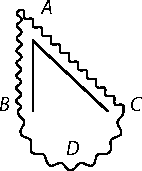
\includegraphics[scale=1]{gesamttex/edit_VIII-4/images/LH_35_10_16_009_d1_009r.pdf}
\edcaption{\edtext{\lbrack\textit{Fig.~1}\rbrack}{%
\lemma{\lbrack\textit{Fig.~1}\rbrack}%
\Cfootnote[nonum]{\indexN{\textls{Stevin} (Stevinus), Simon 1548\textendash1620}%
\textsc{S.~Stevin}, \cite{00196}\textit{De Beghinselen der Weeghconst}, Leiden 1586, S.\;41
(\cite{02084}\textit{SPW} I, S.\;176).}}}
\end{edfigure}
\pstart
\noindent
\edtext{Ex evitatione motus perpetui\indexS{motus perpetuus} sequitur regula\indexS{regula inclinationis planorum} statica inclinationis planorum,\indexS{inclinatio plani}}{%
\lemma{Ex evitatione \lbrack...\rbrack\ planorum}%
\Cfootnote{\cite{00196}a.\,a.\,O., Buch~1, Teil~2, Theor.~XI Prop.~XIX mit Koroll.~I,
S.\;40\textendash42 (\cite{02084}\textit{SPW} I, S.\;174\textendash179).}}
ut ostendit figura adjuncta. 
Nam in ea sunt omnia in aequilibrio,\indexS{aequilibrium}
quia alioqui in quam partem catena\indexS{catena} \textit{BACDB} 
\edtext{super erecto\indexS{planum erectum} \textit{BA} et inclinato\indexS{planum inclinatum}}{%
\lemma{super}%
\Bfootnote{%
\textit{(1)}~erecta \textit{BA} et inclinata
\textit{(2)}~erecto \textit{BA} et inclinato~\textit{L}}}
\textit{AC} posita semel iret, in eam 
\edtext{semper itura}{%
\lemma{semper}%
\Bfootnote{%
\textit{(1)}~iturus
\textit{(2)}~itura~\textit{L}}}
esset, cum semper redeat idem; 
jam \textit{BDC} est in aequilibrio.\indexS{aequilibrium} Ergo et 
\edtext{catenae\indexS{catena}}{\lemma{}\Bfootnote{catenae \textit{erg.~L}}} 
\textit{AB} et \textit{AC} sunt in aequilibrio, quae sunt inter se ut rectae. 
Idem est 
\edtext{\lbrack si\rbrack}{\lemma{}\Bfootnote{si \textit{erg.~Hrsg.}}}
\textit{AB} et \textit{AC} colligantur in unum, velut in sphaeras. 
\pend 
\begin{edfigure}%
\includegraphics[scale=1]{%
gesamttex/edit_VIII-4/images/LH_35_10_16_009_d2_009r.pdf}
\edcaption{\lbrack\textit{Fig.~2}\rbrack}
\end{edfigure}
\pstart 
Eodem modo \textit{EF} et \textit{EG}, catenae sunt in aequilibrio.
Colligatur \textit{EG} in globum \textit{I}. 
Quaeritur ubi is collocari debeat in arcu \textit{EG}, ut 
\edtext{posito \textit{EI} esse}{\lemma{posito}\Bfootnote{%
\textit{(1)}~\textit{EG} esse 
\textit{(2)}~\textit{EI} esse~\textit{L}}} 
catenam pondere carentem,\indexS{catena pondere carens} 
sit pondus \textit{I} in aequilibrio\indexS{aequilibrium}  cum pondere \textit{EF}. 
Id fiet ubi in triangulo elementari\indexS{triangulum elementare} tangens\indexS{tangens} 
\textit{IL} est ad verticalem \textit{IK}, 
\edtext{ut \textit{I},}{\lemma{ut}\Bfootnote{%
\textit{(1)}~\textit{I} ad \textit{EF} \textit{(2)}~\textit{I},~\textit{L}}}
vel \textit{EIG} ad \textit{EF}.
\pend
